\documentclass[10pt,twocolumn,a4paper]{article}
\usepackage[utf8]{inputenc}
\usepackage[french]{babel}
\usepackage[T1]{fontenc}
\usepackage{geometry}
\geometry{top=2.5cm, bottom=2.5cm, left=1.5cm, right=1.5cm}
\usepackage{graphicx}
\usepackage{hyperref}
\usepackage{amsmath}
\usepackage{booktabs} 
\usepackage{float}
\usepackage{microtype}
\raggedbottom
\emergencystretch=1.5em

\title{\textbf{Simulation d'Érosion Hydraulique et Thermique \\ en Temps Réel sur GPU via Compute Shaders}}
\author{
    \textbf{César CHARBEY, Thomas BARASCUD, Jérémy NICOLAS, Lucas PAULO} \\
    Université de Montpellier - Faculté des Sciences \\
    Projet de TER - Encadrant : Nicolas Lutz
}
\date{Année Universitaire 2025-2026}

\begin{document}

\begin{titlepage}
    \centering
    \begin{figure}
        \centering
        
\includegraphics[width=0.4\linewidth]{images/logoUM.png}
    \end{figure}

    \vspace{1cm}
    \textsc{\Large Université de Montpellier}\\[0.2cm]
    \textsc{\large Faculté des Sciences}\\[0.5cm]
    \textsc{\large Master 1 Informatique - Parcours IMAGINE}\\[1.5cm]

    \rule{\linewidth}{0.5mm}\\[0.4cm]
    {\huge \bfseries Simulation d'Érosion Hydraulique et Thermique en Temps Réel sur GPU}\\[0.4cm]
    \rule{\linewidth}{0.5mm}\\[1.5cm]

    \begin{minipage}{0.45\textwidth}
        \begin{flushleft} \large
            \emph{Auteurs :}\\
            César \textsc{Charbey}\\
            Thomas \textsc{Barascud}\\
            Jérémy \textsc{Nicolas}\\
            Lucas \textsc{Paulo}
        \end{flushleft}
    \end{minipage}
    \begin{minipage}{0.45\textwidth}
        \begin{flushright} \large
            \emph{Encadrant :} \\
            Nicolas \textsc{Lutz}
        \end{flushright}
    \end{minipage}\\[2cm]

    \vfill
    {\large Année Universitaire 2025-2026}
\end{titlepage}

\onecolumn
\tableofcontents
\newpage
\listoffigures
\listoftables
\newpage
\twocolumn

% ----------------------------------------------------------------------------------------------------------------------------------------
%Abstract
\begin{abstract}
    La génération procédurale de terrains virtuels réalistes nécessite la simulation de phénomènes physiques complexes s'étalant sur des temps géologiques. Ce document présente la conception et l'implémentation sur carte graphique (GPU), via la technologie des Compute Shaders, du modèle d'érosion hydraulique rapide initialement proposé par Mei et al. \cite{MDH07}. Afin de pallier le manque de détails géométriques inhérent à ces approches, tel que mis en évidence par Schott et al. \cite{SGG24}, nous avons étendu cette architecture en y intégrant une modélisation avancée de l'érosion thermique (éboulements gravitationnels), en nous appuyant sur les travaux de Jákó et Szirmay-Kalos \cite{Jako11}. Nos résultats démontrent qu'il est possible d'augmenter drastiquement le réalisme des pentes abruptes et la distribution sédimentaire, tout en maintenant des performances d'exécution colossales (avoisinant les 960 FPS), prouvant ainsi la viabilité de ce modèle couplé pour des applications interactives exigeantes.
\end{abstract}

% ----------------------------------------------------------------------------------------------------------------------------------------
% Introduction
\section{Introduction}

\subsection{Contexte et Enjeux Industriels}
Dans l'industrie contemporaine du divertissement numérique qu'il s'agisse du jeu vidéo "Triple A", de la réalité virtuelle ou des effets spéciaux cinématographiques la création de mondes ouverts (\textit{Open Worlds}) d'un réalisme saisissant est devenue une exigence fondamentale. L'immersion de l'utilisateur repose en grande partie sur la cohérence visuelle et géologique du terrain. Cependant, sculpter manuellement des environnements de plusieurs dizaines de kilomètres carrés est une tâche titanesque pour les artistes.

C'est ici qu'intervient la génération procédurale, complétée par la simulation physique. Des outils professionnels tels que \textit{Gaea} ou \textit{World Machine} ont prouvé l'utilité de l'érosion pour transformer des bruits mathématiques abstraits en paysages crédibles. Néanmoins, ces solutions reposent souvent sur des calculs hors-ligne (\textit{offline}), brisant le flux créatif des concepteurs.

\subsection{La Problématique de l'Érosion en Temps Réel}
L'apparence organique des chaînes de montagnes, des lits de rivières et des vallées est le résultat de millénaires d'interactions entre les précipitations atmosphériques et la croûte terrestre. Les mouvements d'eau sculptent ces terrains par des processus couplés de dissolution mécanique, de transport hydrodynamique de matière en suspension, et de sédimentation.



Si les méthodes basées sur la mécanique des fluides offrent une fidélité physique incontestable, elles ont historiquement souffert de temps de calcul élevés. Le défi de ce projet de TER est de concevoir une solution capable de simuler ces cycles géologiques complexes en quelques millisecondes.

En nous appuyant sur l'accélération matérielle des Compute Shaders et sur les travaux de Mei et al. \cite{MDH07} et Jákó et al. \cite{Jako11}, nous visons à offrir un laboratoire géomorphologique interactif. Ce dernier ne doit pas seulement être rapide, mais aussi physiquement cohérent, intégrant l'instabilité thermique des sols pour garantir la formation naturelle d'éboulis et de talus.

% ----------------------------------------------------------------------------------------------------------------------------------------
% Etat de l'art
\section{État de l'Art et Positionnement}

La génération de terrains s'est d'abord appuyée sur des approches purement mathématiques, basées sur la superposition de bruits pseudo-aléatoires (bruit de Perlin, Simplex, ou fractales). Si ces algorithmes garantissent une exécution quasi-instantanée et une empreinte mémoire minimale, ils souffrent d'une lacune conceptuelle majeure : un manque inhérent de cohérence géologique. Les paysages ainsi générés sont uniformément vallonnés et fondamentalement dénués de réseaux de drainage, de crêtes acérées ou de dépôt sédimentaire.

\begin{figure}[htbp]
    \centering
    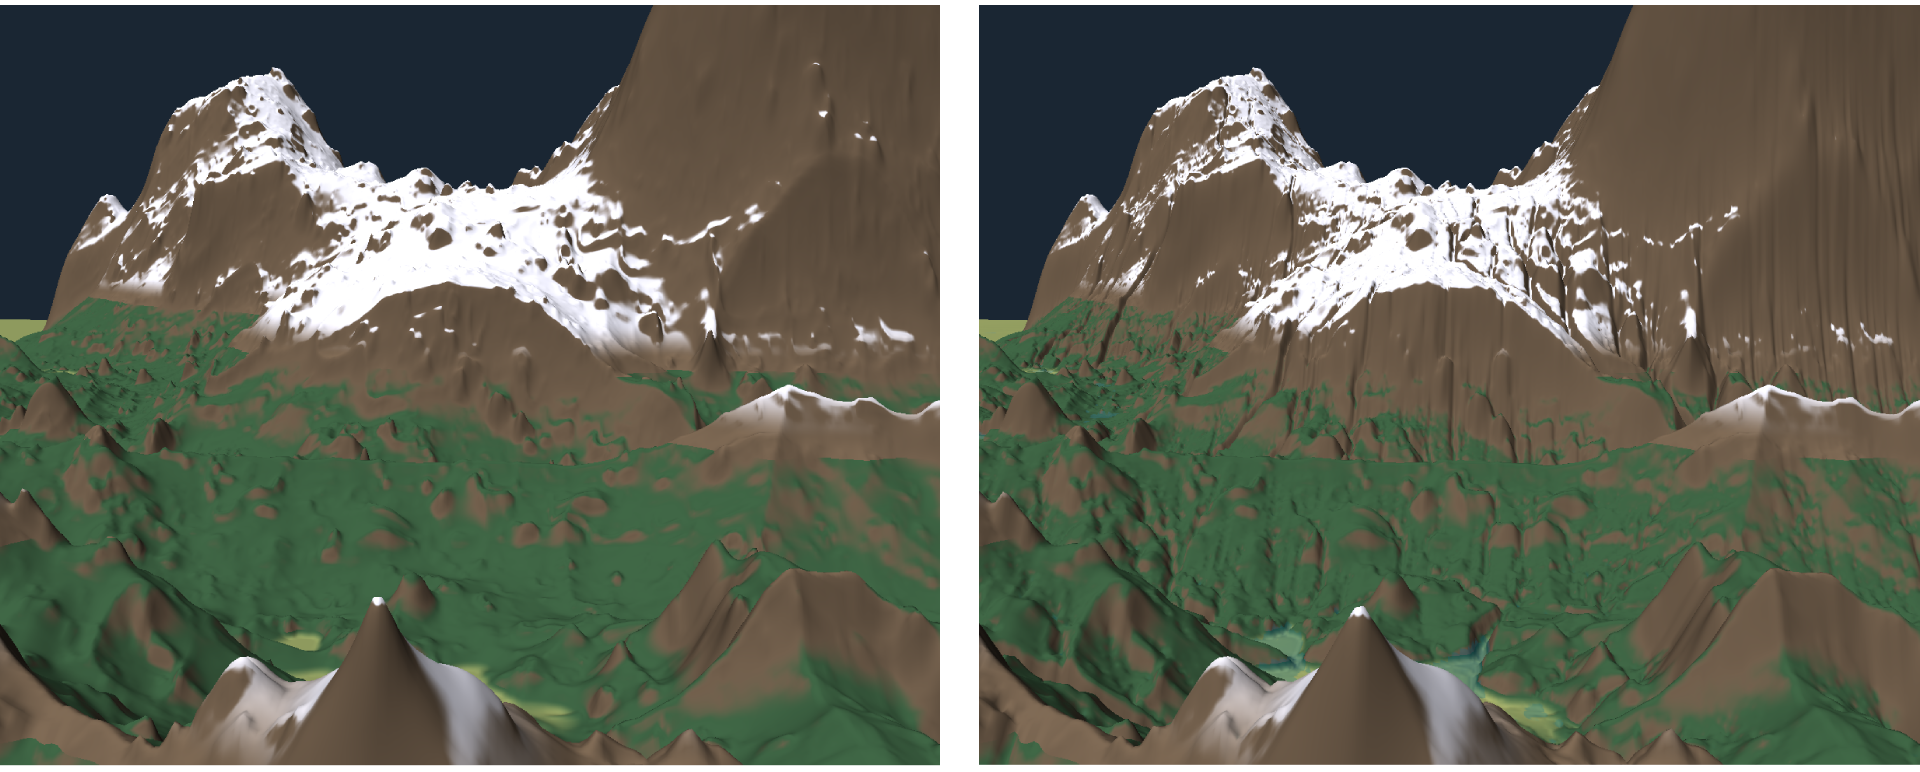
\includegraphics[width=0.95\linewidth]{images/perlin_vs_erosion.png}
    \caption{Comparaison entre une génération procédurale classique par bruit de Perlin (gauche) et un terrain soumis aux forces d'érosion (droite).}
    \label{fig:perlin_vs_erosion}
\end{figure}

Pour insuffler ce réalisme, la recherche s'est orientée vers la simulation des processus d'érosion, posant un défi computationnel de taille.

\subsection{Érosion Hydraulique : Le Paradigme Eulérien}
En 2007, Mei, Decaudin et Hu \cite{MDH07} ont démontré qu'il était possible de simuler l'érosion hydraulique à des fréquences d'affichage interactives. Au lieu de s'engager dans la résolution tridimensionnelle extrêmement lourde des équations de Navier-Stokes, leur modèle exploite une simplification bidimensionnelle : les équations en eaux peu profondes (\textit{Shallow Water Equations}).

Leur approche s'inscrit dans un paradigme \textbf{Eulérien} : l'espace est modélisé sous la forme d'une grille discrète et immuable. Chaque cellule de cette matrice maintient et met à jour un état physique local (hauteur de la roche, hauteur de la colonne d'eau, vélocité du flux, quantité de sédiments). L'écoulement hydrique y est évalué via le "modèle des tuyaux virtuels" (\textit{Virtual Pipe Model}), qui calcule l'accélération de l'eau générée par la différence de pression hydrostatique entre cellules adjacentes. Le transport de la masse sédimentaire est ensuite résolu par advection semi-Lagrangienne rétrograde, garantissant une stabilité inconditionnelle face aux problèmes de divergence numérique.

\subsection{Le Débat Conceptuel : Grilles vs Particules}
L'état de l'art oppose fréquemment ce paradigme Eulérien aux approches \textbf{Lagrangiennes} (systèmes de particules ou \textit{droplet-based erosion}), récemment perfectionnées par Hartley et al. \cite{Hartley24}. Bien que la méthode particulaire excelle visuellement dans le tracé organique de micro-incisions et de ravines abruptes, elle se heurte à des limites matérielles sévères lors de son exécution sur des architectures massivement parallèles (GPU), notamment en raison des conditions de course (\textit{Race Conditions}).

Dans un modèle Lagrangien, la gravité et la topographie forcent naturellement des milliers de particules virtuelles à converger vers les mêmes vallées ou lits de rivières. Sur le plan matériel, cela se traduit par de multiples \textit{threads} concurrents tentant de modifier simultanément la même adresse mémoire (la hauteur d'une cellule spécifique).

Afin d'éviter la corruption des données, la résolution de ces conflits exige l'utilisation d'opérations atomiques (\textit{Atomic Operations} ou \texttt{InterlockedAdd}). Cependant, cette contrainte sérialise localement l'exécution, provoque des conflits d'accès au cache L2 (\textit{cache thrashing}), et anéantit les bénéfices de performance offerts par le parallélisme massif du GPU.

À l'inverse, l'approche Eulérienne, bien que soumise à des artefacts d'advection sur les pentes raides, garantit un schéma d'accès mémoire déterministe et spatialement cohérent (un \textit{thread} = une cellule lue/écrite). Cette garantie de performance et de stabilité justifie pleinement le choix de ce socle algorithmique pour notre implémentation temps réel.
\subsection{La Révolution Matérielle des Compute Shaders}
L'implémentation originelle de Mei \cite{MDH07} était bridée par les limitations matérielles de son époque. L'utilisation contrainte des Fragment Shaders imposait un détournement lourd du pipeline de rastérisation : nécessité de générer de la géométrie fictive, paquetage artificiel des données physiques dans les canaux RGBA, et redondance désastreuse des accès à la mémoire vidéo globale (\textit{VRAM}).

Notre projet tire pleinement parti de la transition architecturale vers les \textbf{Compute Shaders} (introduits avec OpenGL 4.3). Cette technologie s'affranchit du pipeline graphique traditionnel. Les données sont structurées dans des textures ou des \textit{Shader Storage Buffer Objects} (SSBO) accessibles directement en lecture et écriture (\texttt{imageLoad}/\texttt{imageStore}). Bien que la technique du double tamponnage (\textit{ping-pong}) reste indispensable pour figer l'état $t$ lors du calcul de l'état $t+1$, les Compute Shaders permettent l'exploitation de la Mémoire Partagée locale (\textit{Shared Memory}) au sein des \textit{Workgroups}. Ce cache ultra-rapide limite les requêtes redondantes vers la VRAM, déplaçant le goulot d'étranglement de la bande passante vers la capacité de calcul pur de la puce.

\subsection{L'Érosion Thermique comme Nécessité Topologique}
Si le modèle hydraulique creuse des lits de rivières convaincants, il engendre un artefact visuel majeur : l'apparition de falaises parfaitement verticales au bord des flux d'eau, des structures géologiquement instables. Schott et al. \cite{SGG24} soulignent que ces approches manquent de précision et requièrent des processus d'amplification.

Pour répondre à cette problématique, Jákó et Szirmay-Kalos \cite{Jako11} ont mis en évidence la nécessité de coupler l'hydraulique à un modèle d'\textbf{érosion thermique}. Ce processus physique complémentaire simule l'effondrement gravitationnel, le détachement de la roche et la formation d'éboulis dès lors que l'inclinaison locale dépasse l'angle de repos spécifique au matériau.

% ----------------------------------------------------------------------------------------------------------------------------------------
% Explication des modèles mathématiques et physiques
\section{Modélisation de l'Écoulement : Du Continu au Discret}

La simulation de l'érosion repose sur une compréhension précise du mouvement de l'eau. Dans cette section, nous détaillons le passage de la physique théorique "idéale" aux modèles algorithmiques simplifiés nécessaires au temps réel.

\subsection{Le "Graal" de la Physique : Les Équations de Navier-Stokes}
En mécanique des fluides, le modèle de référence absolu est constitué par les \textbf{équations de Navier-Stokes}. Ces équations aux dérivées partielles décrivent comment la vitesse, la pression et la viscosité d'un fluide évoluent dans un espace tridimensionnel.

Mathématiquement, elles garantissent la conservation de la masse et du moment. Cependant, leur résolution en informatique graphique pose trois défis majeurs qui les rendent incompatibles avec le temps réel :

\begin{enumerate}
    \item \textbf{Complexité Volumique :} Pour simuler une rivière de manière réaliste, il faudrait diviser l'espace en une grille 3D. Une résolution de $1024 \times 1024$ sur seulement 100 unités de hauteur représenterait plus de 100 millions de cellules à traiter à chaque milliseconde.
    \item \textbf{Le Solveur de Pression :} Navier-Stokes nécessite la résolution d'une équation de Poisson pour garantir que le fluide est "incompressible" (qu'il ne s'écrase pas sur lui-même). Ce calcul est itératif et extrêmement coûteux en ressources GPU.
    \item \textbf{Instabilité Temporelle :} Pour éviter que la simulation n'explose numériquement, le pas de temps ($\Delta t$) doit être infinitésimal, ce qui interdit toute accélération du temps géologique.
\end{enumerate}

\subsection{La Simplification des Eaux Peu Profondes (SWE)}
Pour atteindre des performances interactives, nous utilisons une version simplifiée : les \textbf{Shallow Water Equations} (SWE). L'hypothèse fondamentale est la suivante : la dimension horizontale du fluide (la largeur de la rivière) est bien plus grande que sa profondeur.

Cette hypothèse permet de négliger la vitesse verticale de l'eau. On passe alors d'un volume 3D complexe à un \textbf{champ de hauteurs 2D}. Le fluide n'est plus un nuage de points dans l'espace, mais une simple valeur de profondeur $d(x,y)$ posée sur chaque cellule de notre grille topographique. C'est cette réduction de dimension (de la 3D à la 2.5D) qui libère la puissance de calcul nécessaire pour atteindre 960 FPS \cite{MDH07}.

\subsection{Le Modèle des Tuyaux Virtuels}
Pour discrétiser ces équations sur GPU, nous utilisons le modèle des \textbf{tuyaux virtuels} de Mei et al. \cite{MDH07}. Chaque cellule est vue comme un réservoir relié à ses voisins par des conduits. La différence de hauteur totale (roche $b$ + eau $d$) crée une pression hydrostatique $\Delta h$ qui génère un flux $f$.

\begin{figure}[htbp]
    \centering
    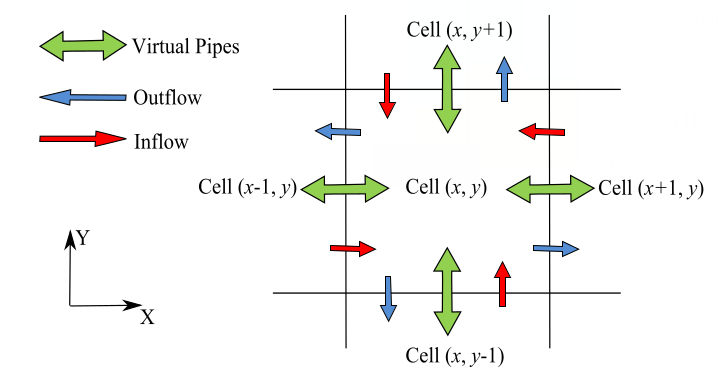
\includegraphics[width=0.7\linewidth]{images/pipe_model.png}
    \caption{Représentation conceptuelle du modèle des tuyaux virtuels gérant les échanges de flux bidimensionnels \cite{MDH07}.}
    \label{fig:pipe_model}
\end{figure}

Le débit sortant vers un voisin est calculé par l'accélération gravitationnelle :
$$ f_{t+\Delta t} = \max \left(0, f_t + \Delta t \cdot A \cdot \frac{g \cdot \Delta h}{l} \right) $$
où $g$ est la gravité, $A$ la largeur du tuyau et $l$ sa longueur. Pour garantir la \textbf{conservation de la masse} et éviter l'apparition d'eau "négative", un facteur de mise à l'échelle $K$ est calculé localement : si la somme des flux sortants excède le volume d'eau de la cellule, les flux sont pondérés uniformément pour ne vider que le volume réel disponible.

% ----------------------------------------------------------------------------------------------------------------------------------------
% Modèle de base
\section{Méthodologie et Ingénierie}

\subsection{Choix Technologiques et Architecture Logicielle}
Pour garantir des performances optimales et un déploiement robuste, le cœur de notre application a été développé en \textbf{C++} standard.

Concernant l'API matérielle, notre choix s'est porté sur \textbf{OpenGL (version 4.3+)} plutôt que sur des plateformes de calcul dédiées (CUDA, OpenCL). Ce choix repose sur un compromis d'ingénierie réfléchi :
\begin{itemize}
    \item \textbf{Compute Shaders vs CUDA :} Utiliser CUDA nous aurait verrouillés dans l'écosystème matériel NVIDIA (rendant l'exécution impossible sur des architectures AMD Radeon). Les Compute Shaders d'OpenGL partagent le \textbf{même contexte mémoire} que les shaders de rendu (Vertex/Fragment). Les textures physiques modifiées par la simulation peuvent donc être directement dessinées à l'écran l'instant suivant.
\end{itemize}

Enfin, l'interface utilisateur, essentielle pour transformer ce projet académique en un véritable outil d'analyse, a été intégrée via la bibliothèque \textbf{Dear ImGui}. Cette bibliothèque permet de lier directement les variables C++ aux éléments d'interface avec un coût de rendu quasi nul, facilitant un débogage interactif.

\subsection{Génération Topographique et Importation}
Le terrain peut être généré procéduralement sur GPU (via un mélange de bruits de type \textit{Ridge} et FBM) ou importé depuis des \textit{heightmaps} réelles. Cette flexibilité permet de tester la robustesse de l'érosion sur des morphologies variées, des pics acérés aux vallées glaciaires lisses.

\subsection{Structures de Données et Stockage GPU}
Pour implémenter les modèles mathématiques décrits précédemment, la simulation utilise une grille de $1024 \times 1024$ cellules. Chaque variable physique est stockée dans une texture OpenGL en virgule flottante 32-bits (\texttt{GL\_R32F} ou \texttt{GL\_RGBA32F}) pour garantir la précision nécessaire aux calculs d'accumulation sédimentaire \cite{MDH07} :

\begin{itemize}
    \item \textbf{Hauteurs ($b, d$) :} Deux canaux stockant la roche et l'eau.
    \item \textbf{Sédiments ($s$) :} Quantité de matière en suspension.
    \item \textbf{Flux ($f$) :} Texture à 4 canaux stockant les débits sortants ($L, R, T, B$) vers les voisins.
    \item \textbf{Vitesse ($\vec{v}$) :} Champ vectoriel 2D déduit du mouvement de l'eau.
\end{itemize}

\begin{figure}[htbp]
    \centering
    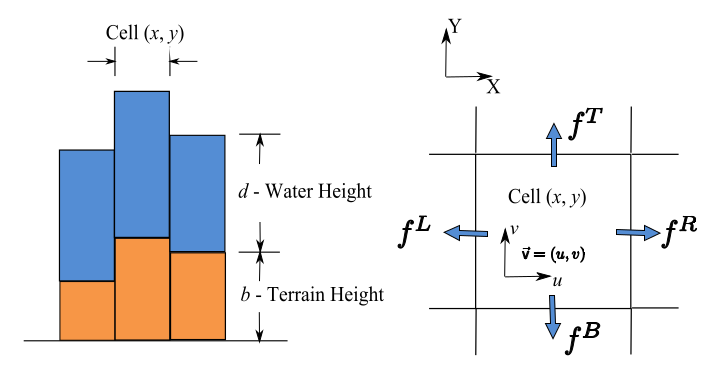
\includegraphics[width=0.8\linewidth]{images/data_structure.png}
    \caption{Organisation des textures GPU et correspondance avec les variables physiques du modèle d'érosion \cite{MDH07}.}
    \label{fig:data_structure}
\end{figure}

L'utilisation des \textbf{Compute Shaders} permet de manipuler ces textures directement via \texttt{imageLoad} et \texttt{imageStore}. Cette approche s'affranchit du pipeline graphique classique et permet d'exécuter les passes physiques (flux, érosion, transport) de manière atomique et ultra-rapide.

\subsection{Améliorations du Modèle de Mei : Apports de Jákó et Szirmay-Kalos}
Bien que le modèle de Mei et al. \cite{MDH07} pose des fondations algorithmiques extrêmement solides pour la simulation Eulérienne en temps réel, son exécution sur des échelles de temps géologiques révèle certaines limites physiques inhérentes : creusement infini des fonds sous-marins, arrachement sédimentaire isotrope, et légères instabilités de la surface hydrique.

Afin de pallier ces défauts et d'élever le réalisme de notre moteur, nous avons outrepassé l'implémentation classique en y intégrant trois corrections physiques majeures issues des travaux postérieurs de Jákó et Szirmay-Kalos \cite{Jako11}. Ces ajouts, intégrés directement au cœur de notre passe d'érosion et de sédimentation (Passe 4), modifient fondamentalement le comportement du fluide :

\begin{itemize}
    \item \textbf{Inhibition de l'érosion en eaux profondes ($l_{max}$) :} Dans le modèle de 2007, un fleuve se jetant dans un lac continue d'éroder le fond marin de manière perpétuelle. Nous avons implémenté un facteur d'atténuation dynamique contraint par la profondeur locale. Lorsque la hauteur de la colonne d'eau dépasse un seuil critique, la capacité de transport s'annule. Ce mécanisme protège naturellement les fonds sous-marins et force le dépôt des sédiments aux embouchures, générant des deltas fluviaux et des hauts-fonds organiques.

    \item \textbf{Collision Hydrologique 3D :} La capacité d'arrachement de la roche ne dépend plus uniquement d'une simple pente bidimensionnelle. L'algorithme calcule désormais la force d'impact via le produit scalaire entre le vecteur de vélocité tridimensionnel du fluide et la normale de la surface heurtée. Une masse d'eau percutant un obstacle géométrique de plein fouet creusera ainsi de manière exponentiellement plus agressive qu'un fluide glissant parallèlement à une pente douce.

    \item \textbf{Couplage Volumétrique Eau-Sédiment :} L'approche originelle omettait le volume physique occupé par la terre en suspension dans l'eau. Nous avons résolu cette incohérence par un couplage strict des états : lorsqu'un volume de roche est arraché, il s'ajoute instantanément à la colonne d'eau locale. Inversement, la déposition sédimentaire abaisse le niveau d'eau. Cette correction de la conservation des masses neutralise les comportements indésirables, garantissant la stabilité absolue de la surface des lacs sur de très longues sessions de simulation.
\end{itemize}

L'intégration de ces contraintes transforme le solveur mathématique de base en une véritable simulation géomorphologique, et ce, avec un coût computationnel supplémentaire rendu totalement invisible par l'architecture des Compute Shaders.

\subsection{Érosion Thermique Avancée : Dureté Locale et Voisinage de Moore}
La modélisation de l'érosion thermique sur une grille discrète soulève généralement deux problématiques géométriques majeures : l'apparition de structures pyramidales artificielles (lorsque l'évaluation se restreint à un voisinage de von Neumann à 4 directions) et un aspect "plastique" globalisé (causé par l'utilisation d'un angle de talus constant sur l'ensemble du domaine).

Pour contourner ces défauts, notre algorithme intègre directement le modèle avancé de Jákó et Szirmay-Kalos \cite{Jako11}. L'instabilité mécanique et le transfert de sédiments y sont évalués sur un voisinage de Moore (8 directions), permettant la formation de cônes d'éboulis organiques et parfaitement circulaires. Plutôt que de déplacer la matière de manière séquentielle et gloutonne, nous avons appliqué le paradigme Eulérien des "tuyaux virtuels" au substrat rocheux lui-même.

\begin{figure}[htbp]
    \centering
    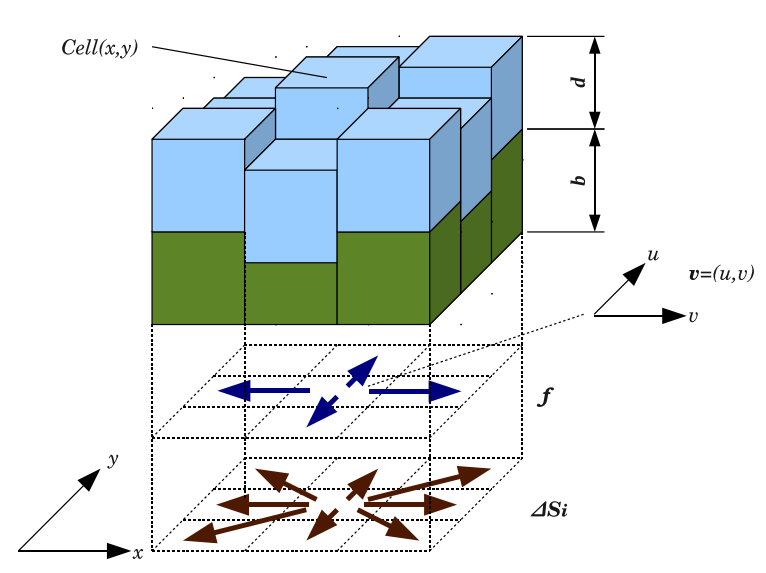
\includegraphics[width=0.60\linewidth]{images/thermal.png}
    \caption{Comparaison géométrique du modèle des tuyaux virtuels appliqué à l'écoulement d'eau (voisinage de von Neumann à 4 directions, flèche bleue) et à l'éboulement thermique des sédiments (voisinage de Moore à 8 directions, flèche rouge).}
    \label{fig:thermal_pipe_model}
\end{figure}

Une première passe calcule les volumes de terre devant s'effondrer et les stocke sous forme de flux directionnels virtuels, tandis qu'une seconde passe synchronise la nouvelle topologie en additionnant ces flux. Cette architecture en deux temps résout élégamment les dépendances d'écriture tout en garantissant la conservation stricte du volume topologique.

De plus, afin de briser l'homogénéité visuelle typique des simulations standards (l'effet plastique), la tangente de l'angle de talus est modulée en chaque point par un coefficient de dureté locale $R(x,y)$. Ce coefficient est généré dynamiquement sur le GPU en combinant l'élévation (la roche en haute altitude étant physiquement plus dense) et un bruit pseudo-aléatoire simulant l'hétérogénéité des strates géologiques. Les sommets peuvent ainsi soutenir des falaises presque verticales, tandis que les vallées s'affaissent en pentes douces, créant une richesse géomorphologique inatteignable avec un angle de repos statique.

\begin{figure}[htbp]
    \centering
    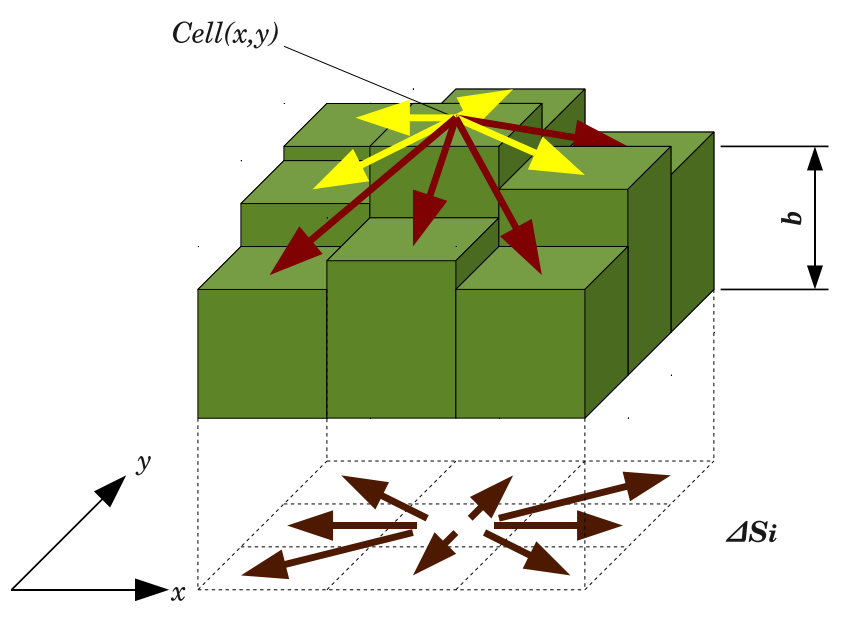
\includegraphics[width=0.60\linewidth]{images/pipes_thermal_erosion.png}
    \caption{Mécanisme des tuyaux virtuels appliqué à l'érosion thermique. Les transferts de sédiments (flèches rouges) s'effectuent exclusivement vers les cellules voisines dont le dénivelé excède l'angle de talus local. À l'inverse, l'éboulement est mathématiquement inhibé (flèches jaunes) vers les zones considérées comme géologiquement stables.}
    \label{fig:thermal_exemple}
\end{figure}

\subsection{Stabilité Numérique et Condition CFL}
Un défi inhérent aux solveurs de fluides explicites réside dans leur instabilité si le pas de temps d'intégration ($\Delta t$) est inadapté à la vélocité maximale du fluide. Si l'eau se déplace sur une distance supérieure à la taille d'une cellule en une seule itération, le modèle mathématique s'effondre. Pour éviter ces explosions numériques, nous avons implémenté une vérification stricte de la condition de Courant-Friedrichs-Lewy (CFL) :
$$ \Delta t \le \frac{\Delta x}{v_{max}} $$
Notre interface ImGui avertit l'utilisateur de manière dynamique si les paramètres de gravité ou d'apport d'eau nécessitent une réduction du pas de temps pour maintenir la cohésion mathématique de la simulation.

\subsection{Implémentation du Pipeline et Gestion Mémoire}
La boucle de calcul est exécutée par des groupes de travail (\textit{Workgroups}) matériels de $16 \times 16$ \textit{threads}, une taille empiriquement optimale pour maximiser l'occupation des cœurs de calcul de l'architecture graphique.

Pour pallier les problèmes de concurrence en écriture inévitables sur une grille globale, notre architecture repose sur un \textbf{double tamponnage} (\textit{ping-pong buffering}). Les textures stockant les hauteurs, l'eau et les sédiments sont dupliquées. À l'itération $i$, les shaders lisent l'état figé dans les tampons \texttt{READ} et inscrivent les résultats dans les tampons \texttt{WRITE}.

L'intégrité de la simulation est assurée par l'injection de barrières de mémoire (\texttt{glMemoryBarrier\allowbreak(GL\_\allowbreak SHADER\_\allowbreak IMAGE\_\allowbreak ACCESS\_\allowbreak BARRIER\_\allowbreak BIT)}) entre chaque appel de noyau. Cette instruction force le GPU à purger les données de son cache L1/L2 vers la mémoire globale avant d'autoriser le shader suivant à débuter. Grâce à ce séquençage en "aller-retour" (du tampon \texttt{READ} vers \texttt{WRITE}, puis inversement), l'état physique final est toujours garanti d'être valide et disponible dans le tampon \texttt{READ} pour le rendu visuel de la trame courante.

\begin{figure}[htbp]
    \centering
    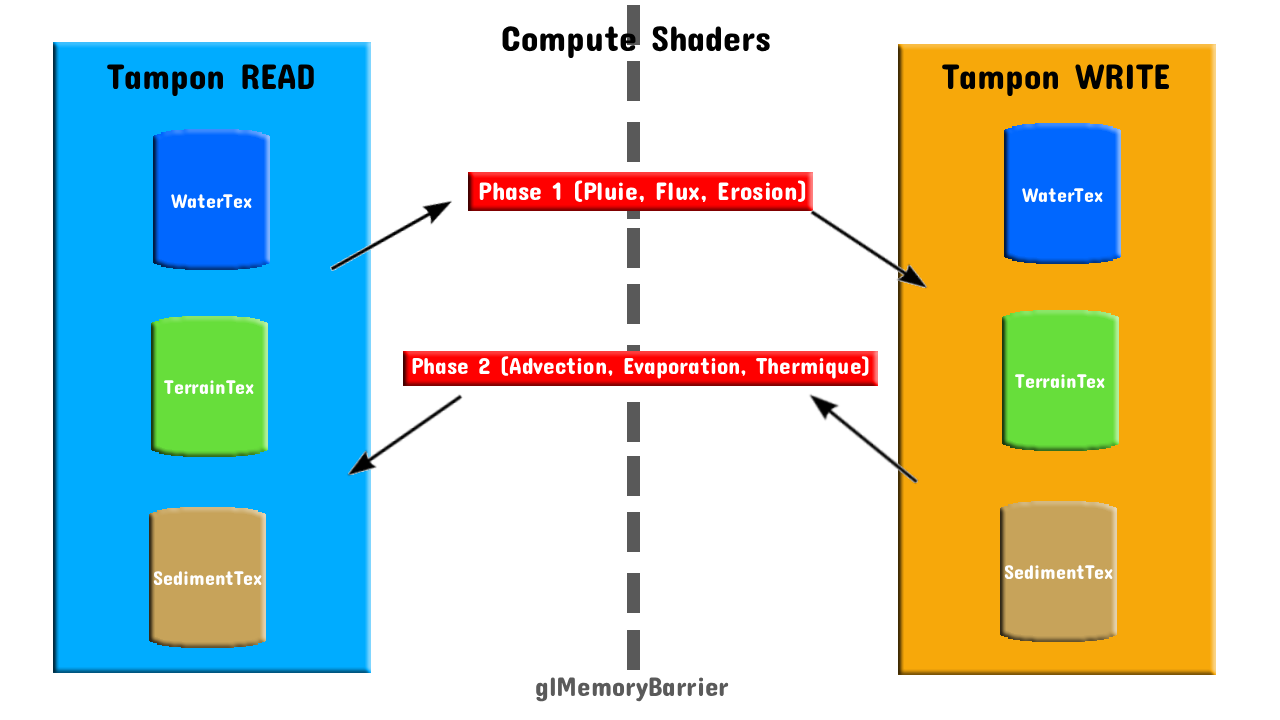
\includegraphics[width=0.9\linewidth]{images/ping_pong.png}
    \caption{Architecture du double tamponnage : les passes physiques écrivent dans le tampon temporaire (WRITE), tandis que les passes de post-traitement rapatrient l'état final dans le tampon principal (READ), sous la protection des barrières mémoire.}
    \label{fig:ping_pong}
\end{figure}

\subsection{Le Pipeline de Rendu Graphique}
Calculer l'érosion d'une grille de $1024 \times 1024$ cellules à haute fréquence n'a de sens que si le moteur graphique est capable d'afficher ces plus de deux millions de triangles à la même vitesse. Pour ne pas brider la simulation physique, notre pipeline de rendu a été drastiquement optimisé.

\paragraph{Déplacement des Sommets sur GPU (\textit{Vertex Displacement}) :}
Plutôt que de faire lire le tableau des hauteurs par le CPU pour générer la géométrie, nous envoyons à la carte graphique, une unique fois lors de l'initialisation, un maillage plan régulier (\textit{Flat Grid}) stocké dans un \textit{Vertex Buffer Object} (VBO). Lors de la phase de rendu, le \textbf{Vertex Shader} lit directement la texture des hauteurs $b$ (roche) et $d$ (eau) produite par la simulation physique, et déplace la coordonnée $Y$ de chaque sommet à la volée.

\paragraph{Calcul des Normales à la Volée :}
Pour que la lumière réagisse au relief de manière réaliste, chaque sommet doit posséder un vecteur normal. Au lieu de dédier une passe de Compute Shader supplémentaire pour calculer et stocker ces normales (ce qui consommerait de la bande passante mémoire), nous les calculons dynamiquement dans le \textbf{Fragment Shader}. En échantillonnant l'altitude des pixels voisins directement dans la texture de hauteur via la fonction \texttt{texelFetch}, le shader déduit le gradient local et calcule le produit vectoriel pour obtenir la normale parfaite. Cette approche permet d'économiser la bande passante mémoire qui est le véritable goulot d'étranglement de notre application.

\paragraph{Ombrage et Coloration Topographique (\textit{Shading}) :}
La couleur finale du terrain est générée procéduralement. Le shader interpole différentes textures (herbe, roche, neige) non seulement en fonction de l'altitude, mais surtout en fonction de la pente (déduite de la normale calculée). Ainsi, une falaise abrupte apparaîtra rocheuse même à basse altitude, tandis qu'un plateau sera couvert de sédiments ou de végétation. La couche d'eau, quant à elle, bénéficie d'un ombrage transparent teinté de bleu dont l'opacité dépend directement de la valeur de la colonne d'eau $d$, rendant l'accumulation dans les lacs visuellement distincte des minces ruisseaux.

% ----------------------------------------------------------------------------------------------------------------------------------------
% Différentes passes de notre projet
\section{Détails de l'Implémentation du Pipeline}

Notre pipeline d'érosion a été segmenté en huit passes de Compute Shaders distinctes, formant une boucle itérative où chaque étape dépend des résultats de la précédente. Pour pallier les manques du modèle historique, nous avons enrichi chaque phase par des modèles physiques plus récents.

\paragraph{1. Apport Hydrique : Pluie et Sources (\texttt{water\_increment.glsl}) :}
Cette première étape injecte l'énergie initiale (le volume d'eau) dans notre système. La hauteur de la colonne d'eau $d$ de chaque cellule est mise à jour en intégrant l'apport hydrique sur le pas de temps $\Delta t$. Cet apport se décompose en deux mécanismes distincts :
\begin{itemize}
    \item \textbf{Précipitation globale :} Une pluie uniforme $r$ arrose l'intégralité de la topographie selon l'équation $d_{t+\Delta t} = d_t + (\Delta t \cdot r)$. Au-delà de l'aspect géologique, le maintien de cette nappe d'eau globale est une nécessité mathématique. En mécanique des fluides sur grille, une épaisseur d'eau nulle ($d = 0$) entraîne un risque de division par zéro lors du calcul ultérieur de la vitesse ($v = \text{débit} / d$). La pluie garantit ainsi une fine pellicule hydrique permanente, prévenant l'apparition de ces singularités numériques.
    \item \textbf{Sources locales (Rivières) :} Afin d'offrir un contrôle interactif, le simulateur permet à l'utilisateur d'injecter un débit d'eau massif à des coordonnées ciblées. Mathématiquement, cela se traduit par une addition scalaire contrainte dans un rayon défini, simulant la résurgence d'une source souterraine et permettant de diriger intentionnellement le creusement d'une vallée.
\end{itemize}

\paragraph{2. Calcul des Flux par Tuyaux Virtuels (\texttt{flux\_compute.glsl}) :}
Cette passe constitue le moteur hydrodynamique du simulateur. Elle évalue la quantité d'eau qui doit transiter entre chaque cellule et son voisinage de von Neumann (les 4 directions cardinales), en s'appuyant sur le modèle de Mei et al. \cite{MDH07}. L'évaluation se déroule en trois étapes :
\begin{itemize}
    \item \textbf{Pression hydrostatique :} L'algorithme calcule d'abord la différence d'altitude absolue $\Delta h = (b_{local} + d_{local}) - (b_{voisin} + d_{voisin})$. Si $\Delta h > 0$, la gravité exerce une pression poussant le fluide vers la cellule voisine.
    \item \textbf{Accélération inertielle :} L'écoulement n'est pas instantané ; l'eau possède une inertie. Le flux sortant $f$ est mis à jour en ajoutant la nouvelle accélération au flux de l'itération précédente :
          $$ f_{t+\Delta t} = \max \left( 0, f_t + \Delta t \cdot A \frac{g \cdot \Delta h}{l} \right) $$
          L'utilisation de la fonction $\max(0, \dots)$ est ici cruciale : elle garantit un écoulement strictement unidirectionnel, empêchant mathématiquement l'eau de remonter un tuyau à contre-courant. $A$ représente la section transversale du flux, $g$ la constante gravitationnelle, et $l$ la distance inter-cellulaire.
    \item \textbf{Conservation de la masse (Facteur $K$) :} Sur une grille discrète, une forte pente combinée à un pas de temps $\Delta t$ trop grand pourrait théoriquement forcer une cellule à expulser un volume d'eau supérieur à celui qu'elle contient réellement. Pour prévenir cette aberration physique (qui engendrerait une hauteur d'eau négative), le système calcule un scalaire de sécurité $K$. Si la somme des flux sortants excède le volume disponible, $K$ pondère uniformément les quatre vecteurs de sortie vers le bas. Cela garantit une conservation de masse absolue et une stabilité inconditionnelle du solveur de fluides.
\end{itemize}

\paragraph{3. Mis à jour du niveau d'eau(\texttt{water\_update.glsl}) :}
Une fois les flux validés, cette passe synchronise l'état physique de la cellule selon trois axes :
\begin{itemize}
    \item \textbf{Mise à jour hydrique :} La nouvelle hauteur d'eau $d_{t+\Delta t}$ est déduite par une simple somme algébrique du volume préexistant, du volume entrant depuis le voisinage, et du volume sortant.
    \item \textbf{Inférence du champ vectoriel :} Dans le modèle des Shallow Water, la vitesse $\vec{v} = (u,v)$ n'est pas stockée directement comme une variable indépendante, elle est \textit{inférée}. L'algorithme calcule le débit net traversant la cellule sur l'axe $X$ (moyenne des flux gauche/droite) et l'axe $Y$ (moyenne haut/bas). En divisant ce vecteur de débit par la hauteur d'eau moyenne locale, on obtient le vecteur vitesse tridimensionnel du fluide.
    \item \textbf{Friction et Rugosité spatiale :} Nous avons introduit un coefficient de friction dans le calcul de cette vitesse. Sans cette dissipation d'énergie cinétique, la gravité forcerait l'eau dévalant une falaise à atteindre une vitesse infinie (violant la condition CFL). Ce frein simule la rugosité du terrain (similaire au coefficient de Manning en hydrologie), garantissant un temps de résidence suffisant du fluide sur les pentes abruptes pour que l'érosion puisse s'y opérer.
\end{itemize}

\paragraph{4. Érosion et Sédimentation Avancées (\texttt{erosion\_deposition.glsl}) :}
Cette passe régit le transfert de masse entre la roche dure (le substrat $b$) et la terre en suspension (le sédiment $s$). Le transfert est dicté par la \textbf{capacité de transport} $C$, représentant la charge sédimentaire maximale que l'eau peut porter avant saturation.
\begin{itemize}
    \item \textbf{Évaluation de la Capacité :} Suivant les travaux de Jákó \cite{Jako11} introduits en Section 3.4, $C$ est pondéré par l'impact géométrique (produit scalaire) et freiné en eaux profondes ($l_{max}$) pour protéger les fonds marins :
          $$ C = K_c \cdot \max(0.15, -\vec{v}_{3D} \cdot \vec{n}) \cdot |\vec{v}| \cdot l_{max} $$
    \item \textbf{Cinétique de Transfert :} L'altération n'est pas instantanée. Si l'eau est sous-saturée ($C > s$), elle arrache de la roche selon un taux de dissolution $K_s$ : $\Delta s = K_s \cdot (C - s)$. Si l'eau est sur-saturée ($C < s$), elle dépose le surplus selon un taux de sédimentation $K_d$ : $\Delta s = K_d \cdot (s - C)$. La topologie $b$ et la charge sédimentaire $s$ sont mises à jour par ces deltas.
\end{itemize}

\paragraph{5. Transport Sédimentaire par Advection (\texttt{sediment\_transport.glsl}) :}
Une fois arrachés au sol, les sédiments $s$ ne restent pas immobiles : ils sont charriés par le courant. C'est le phénomène physique d'\textbf{advection}. La difficulté majeure sur une grille fixe (paradigme Eulérien) est de déplacer cette matière continue d'une case à l'autre sans créer de "trous" ou d'accumulations aberrantes.

Pour y parvenir, nous utilisons la méthode d'advection \textbf{semi-Lagrangienne rétrograde} \cite{MDH07}. Plutôt que d'essayer de calculer où vont aller les sédiments (ce qui s'avère instable), l'algorithme "regarde en arrière" (\textit{backtracing}). Ce mécanisme se déroule en trois étapes :
\begin{itemize}
    \item \textbf{Ciblage spatial :} Pour chaque cellule $(x,y)$, l'algorithme lit le vecteur vitesse actuel de l'eau $\vec{v}$.
    \item \textbf{Remontée du temps :} Il remonte virtuellement le courant "dans le passé" d'une durée $\Delta t$ pour trouver les coordonnées exactes d'où provient l'eau qui arrive actuellement dans la cellule.
    \item \textbf{Échantillonnage :} Comme cette coordonnée d'origine tombe rarement au centre parfait d'une case de la grille, l'algorithme calcule la quantité de sédiments présente à cet endroit précis en effectuant une moyenne pondérée des 4 cases les plus proches (\textbf{interpolation bilinéaire}). La cellule $(x,y)$ s'approprie ensuite cette nouvelle valeur.
\end{itemize}

\paragraph{6. Évaporation et Conditions aux Limites (\texttt{evaporation.glsl}) :}
Le cycle hydrologique s'achève par l'extraction de l'eau hors du système. Cette étape est indispensable pour garantir un équilibre volumétrique sur le long terme face aux précipitations continues de la Passe 1. Cette extraction s'opère selon deux mécanismes distincts :
\begin{itemize}
    \item \textbf{Évaporation différentielle :} La hauteur d'eau diminue proportionnellement à un taux $K_e$, selon l'équation de décroissance $d_{t+\Delta t} = d_t \cdot (1 - K_e \cdot \Delta t)$. Au-delà de cette constante, nous avons implémenté une heuristique d'évaporation pondérée par la cinématique : l'eau stagnante ($|\vec{v}| \approx 0$) s'évapore mathématiquement plus vite que l'eau en mouvement. Ce choix d'ingénierie favorise l'assèchement naturel des flaques isolées et évite au GPU de calculer inutilement la physique de micro-volumes d'eau perpétuels, tout en préservant le débit des rivières principales.
    \item \textbf{Ouverture du domaine (Conditions de Dirichlet) :} Sur une grille mathématique finie, l'accumulation de fluides aux frontières génère des barrages artificiels irréalistes. Pour contourner ce problème, cette passe impose des \textbf{conditions aux limites de Dirichlet} de valeur nulle sur tout le périmètre de la carte. En forçant systématiquement la hauteur d'eau $d$ et la charge sédimentaire $s$ à zéro sur les bords de la texture, nous transformons la grille fermée en un système ouvert. La matière peut ainsi s'évacuer définitivement, simulant l'écoulement naturel d'un bassin versant vers un océan infini.
\end{itemize}

\paragraph{7. Évaluation de l'Instabilité Gravitationnelle (\texttt{thermal\_flux.glsl}) :}
Indépendamment de l'action de l'eau, cette passe simule les éboulements terrestres (érosion thermique). L'algorithme transpose le concept de "tuyaux virtuels" à la roche, en l'évaluant cette fois sur un voisinage de Moore (8 directions) \cite{Jako11} pour éviter l'apparition de montagnes pyramidales artificielles (artefact courant des voisinages à 4 directions). L'évaluation suit ces règles :
\begin{itemize}
    \item \textbf{Dureté et Angle de Talus :} L'algorithme évalue l'excès de pente de chaque cellule par rapport à ses voisines. Le seuil de rupture n'est pas uniforme : il est défini par un coefficient de dureté locale $R(x,y)$, généré dynamiquement par un bruit spatial. Cette hétérogénéité permet à certaines zones de soutenir des falaises presque verticales (roche dure), tandis que d'autres s'affaissent (roche friable).
    \item \textbf{Distribution des Flux :} Si l'inclinaison dépasse l'angle de repos $R(x,y)$, le volume de terre instable est calculé puis réparti proportionnellement dans 8 flux directionnels virtuels, privilégiant les pentes les plus raides.
    \item \textbf{Inhibition Hydrique :} L'éboulement est mathématiquement inhibé vers les cellules abritant un flux d'eau. Cette contrainte est géologiquement cruciale : elle protège les ravins et empêche les berges de s'effondrer instantanément pour combler les lits de rivières fraîchement creusés par la Passe 4.
\end{itemize}

\paragraph{8. Synchronisation (\texttt{thermal\_apply.glsl}) :}
La topologie globale est définitivement mise à jour lors de cette dernière itération. Le découpage de l'érosion thermique en deux étapes distinctes (Calcul puis Application) répond à une contrainte architecturale critique du GPU : la gestion de la concurrence mémoire.
\begin{itemize}
    \item \textbf{Résolution des Conditions de Course :} Dans un modèle massivement parallèle, si un \textit{thread} (une cellule) tentait de "pousser" directement de la terre vers ses voisins, de multiples \textit{threads} pourraient écrire simultanément à la même adresse mémoire, corrompant irrémédiablement la topologie (\textit{race condition}).
    \item \textbf{Approche par Rassemblement :} Pour contourner ce souci sans recourir à des opérations atomiques (qui sérialiseraient les calculs et anéantiraient nos performances de 960 FPS), cette passe opère en lecture locale. Chaque cellule lit en sécurité les flux thermiques que ses 8 voisins ont préparés \textit{pour elle}, et calcule son propre bilan : $b_{t+1} = b_t - \sum \text{flux\_sortants} + \sum \text{flux\_entrants}$. Ce \textit{design pattern} garantit un déterminisme absolu et une conservation topologique parfaite au gramme près.
\end{itemize}

% ----------------------------------------------------------------------------------------------------------------------------------------
% Limites Numériques
\subsection{Limites Numériques et Conditions aux Frontières}
La transposition d'équations continues sur une grille discrète impose inévitablement des compromis mathématiques. Si notre architecture garantit la conservation stricte du volume hydrique, le transport sédimentaire et la gestion du domaine soulèvent des défis inhérents au paradigme Eulérien.

Le premier compromis majeur concerne \textbf{la non-conservation de la masse sédimentaire}. La passe d'advection semi-Lagrangienne (Passe 5), bien que reconnue pour sa stabilité absolue face aux courants rapides, n'est pas strictement conservative. Dans les zones de forte divergence du champ vectoriel (typiquement les crêtes), de multiples cellules adjacentes ciblent la même cellule source lors du \textit{backtracing}. Ce phénomène duplique numériquement la charge sédimentaire.
Résoudre ce défaut nécessiterait d'abandonner l'advection semi-Lagrangienne au profit de schémas strictement conservatifs (comme la méthode \textit{BFECC} ou les grilles MAC), dont le coût computationnel ruinerait les performances interactives du GPU. Nous avons donc accepté cette dérive non-physique comme un mal nécessaire du temps réel, simplement mitigée par l'application d'un infime facteur de dissipation globale évitant l'emballement du système sur les très longues sessions.

Le second défi est lié à la nature finie de la grille de simulation : la gestion des \textbf{conditions aux limites}. Initialement traitée comme un système fermé, la matrice empêchait la matière de s'échapper, conduisant à une accumulation inexorable contre les frontières et à la formation de barrages artificiels noyant la topologie.
Contrairement au problème d'advection, cette limite géométrique a pu être résolue de manière élégante en imposant des \textbf{conditions de Dirichlet nulles} sur le périmètre extérieur. Les cellules bordant la carte agissent désormais comme des "drains" continus, où la hauteur d'eau et les sédiments sont systématiquement forcés à zéro en fin de cycle. Cette modification transforme le domaine en un système ouvert, simulant l'écoulement naturel d'un bassin versant vers un océan virtuel infini.


% ----------------------------------------------------------------------------------------------------------------------------------------
% Résultats et Évaluation
\section{Résultats et Évaluation}
Afin de quantifier de manière irréfutable les bénéfices de l'architecture Compute Shader, nous avons développé une implémentation rigoureusement équivalente s'exécutant de manière séquentielle sur le processeur (CPU). Ce programme en C++ natif nous sert de \textit{baseline} absolue pour mesurer le ratio d'accélération sur des \textit{heightmaps} d'entrée identiques.

Notre évaluation intègre les mesures documentées par Mei et al. en 2007 \cite{MDH07} (GeForce 8800 GTX), ainsi que les résultats plus récents de Jákó et Szirmay-Kalos en 2011 \cite{Jako11} obtenus sur une architecture ATI Radeon HD4870. À titre de comparaison, le modèle de 2011 atteignait un temps de cycle global de 15,47\,ms pour une grille de résolution similaire ($1024 \times 1014$) \cite{Jako11}. Nos propres mesures ont été isolées via les \textit{Timestamp Queries} d'OpenGL sur une plateforme composée d'un processeur AMD Ryzen 5 2600 et d'une carte graphique AMD Radeon RX 5700.

\begin{table}[htbp]
    \centering
    \resizebox{\columnwidth}{!}{%
        \begin{tabular}{lcccc}
            \toprule
            \textbf{Étape de calcul} & \textbf{Mei (2007)} & \textbf{Jákó (2011)} & \textbf{Notre CPU}   & \textbf{Notre GPU} \\
            \midrule
            Sim. Physique (Eau)      & 6.65 ms             & N/A                  & 898.244 ms           & 0.408 ms           \\
            Érosion Thermique        & N/A                 & N/A                  & 821.458 ms           & 0.223 ms           \\
            Rendu Visuel             & 10.31 ms            & N/A                  & 3.227 ms             & 0.407 ms           \\
            \midrule
            \textbf{Temps de Cycle}  & \textbf{16.95 ms}   & \textbf{15.47 ms}    & \textbf{1722.929 ms} & \textbf{1.037 ms}  \\
            \bottomrule
        \end{tabular}%
    }
    \caption{Tableau comparatif des performances (Résolution : $1024 \times 1024$). Les données historiques \cite{MDH07, Jako11} servent de référentiels. Un cycle de 1.037\,ms correspond à une fréquence théorique de 964 images par seconde (FPS).}
    \label{tab:perf}
\end{table}

L'analyse de ces métriques illustre un saut technologique majeur. L'implémentation CPU est terrassée par la complexité algorithmique du voisinage de Moore (8 directions) et les calculs de collision 3D, aboutissant à un temps de cycle critique de 1,72\,seconde. Ce délai rend toute interaction impossible sur processeur (0,58 FPS).

Le basculement sur GPU via Compute Shaders pulvérise ces limitations, ramenant la boucle complète à seulement 1,037\,ms. Le facteur d'accélération global entre notre implémentation CPU et GPU atteint ainsi le ratio colossal de \textbf{1661x}. L'optimisation est particulièrement visible sur l'érosion thermique : malgré la complexité du modèle de Jákó (calcul de flux directionnels et dureté locale), le GPU exécute cette tâche en 0,223\,ms soit une accélération de 3680x face au CPU). Ces résultats prouvent que l'architecture moderne permet d'exécuter des modèles physiques autrefois coûteux (\cite{MDH07, Jako11}) en une fraction de milliseconde.

\subsection{Interactivité et Découplage Temporel}
Cette colossale réserve de puissance (framerate théorique frôlant les 960~FPS) nous a permis d'implémenter un découplage temporel profond entre le moteur physique et le moteur de rendu. L'utilisateur peut, via l'interface ImGui, ordonner l'exécution de multiples itérations physiques (\texttt{ITERATIONS\_PER\_FRAME}, paramétrable jusqu'à 10) pour chaque image affichée à l'écran.

Afin de donner une échelle de grandeur à cette performance, nous avons introduit un facteur de conversion vers le temps géologique. En considérant qu'une seconde de temps physique simulé équivaut à 10\,000 ans d'érosion naturelle, notre simulateur permet de compresser les millénaires de manière fulgurante. Avec un pas de temps $\Delta t = 0,0015$, chaque itération fait avancer l'érosion de 15~ans. À son paramétrage maximal de 10~itérations par trame, l'application calcule 150~années géologiques par image. Ainsi, une seule seconde de simulation en temps réel, standardisée à 60~FPS, permet d'écouler \textbf{9\,000 années géologiques} (un chiffre qui s'envole à plus de 144\,000 années par seconde si le framerate est débridé).

Ce mécanisme permet d'observer en quelques minutes des processus qui nécessiteraient normalement des millions d'années, comme le creusement de canyons profonds ou l'aplanissement de massifs montagneux. L'interface offre de surcroît la possibilité d'altérer les constantes physiques ou de déplacer des sources de rivières à la volée, transformant le programme en un puissant laboratoire géomorphologique interactif où l'utilisateur navigue fluidement à travers les époques.

% -----------------------------------------------------------------------------------------------------------------------------------------
% Discussion
\section{Discussion et Analyse Critique}
Si les métriques brutes valident l'efficacité computationnelle de notre architecture sur GPU, une analyse critique est indispensable pour évaluer la viabilité globale du modèle face aux standards académiques et industriels actuels.

\subsection{Biais Matériel et Goulets d'Étranglement}
Le ratio d'accélération de 1661x mesuré face à notre implémentation CPU est spectaculaire, mais il convient de l'analyser avec prudence. Les temps de cycle documentés par Mei et al. en 2007 (16,95\,ms) \cite{MDH07} et Jákó en 2011 (15,47\,ms) \cite{Jako11} ont été obtenus sur des architectures matérielles (GeForce 8800 GTX et Radeon HD4870) dont la puissance brute et la bande passante mémoire sont non comparables avec notre plateforme de test contemporaine (Radeon RX 5700).

Afin d'éprouver les limites de notre architecture et d'identifier le véritable goulet d'étranglement matériel, nous avons mené un test de charge (\textit{stress-test}) empirique sur une topologie massive de $8192 \times 8192$ cellules (soit plus de 67 millions de sommets gérés simultanément, représentant une multiplication par 64 de l'empreinte mémoire).

Sur cette échelle s'apparentant à un environnement de monde ouvert (\textit{Open World}), le temps de cycle grimpe à 56,03\,ms (soit 17,4 FPS), réparti entre la physique hydrique (28,34\,ms), l'érosion thermique (15,96\,ms) et le rendu visuel (11,72\,ms). Bien que la performance de calcul pure encaisse cette multiplication par 64 de manière quasi-linéaire, la chute du framerate sous le seuil du temps réel interactif (60 FPS) met en exergue la saturation de la bande passante mémoire (\textit{Memory Bandwidth}). Sur de telles résolutions, les allers-retours constants entre la VRAM et les cœurs de calcul lors du \textit{ping-pong buffering} saturent le bus matériel. Cette limite physique démontre que pour un déploiement industriel à très grande échelle, il serait impératif d'abandonner l'évaluation globale de la grille au profit d'une architecture par tuiles dynamiques (\textit{Tile-based processing}) ou par niveaux de détails (\textit{Clipmaps}).

\subsection{Validation Morphologique Qualitetive}
Au-delà de la performance, le réalisme géologique était le second enjeu de ce projet. Le modèle original de Mei, s'il trace des réseaux fluviaux cohérents, a tendance à générer des "trous" (des canyons d'un pixel de large et infiniment profonds).

L'intégration du modèle de Jákó (érosion thermique sur voisinage de Moore et dureté spatiale) a permis d'atténuer ces artefacts. Visuellement, l'ajout des éboulements gravitationnels transforme ces aiguilles instables en vallées en "V" beaucoup plus naturelles, flanquées de cônes d'éboulis à leur base. Cependant, le paradigme Eulérien sur grille 2.5D limite l'expressivité de ces formations : l'impossibilité mathématique d'avoir deux valeurs $Y$ pour un même couple $(X,Z)$ interdit formellement la création de grottes ou de surplombs rocheux, limitant la génération à des paysages de type "vue aérienne".

\subsection{Positionnement face à l'Industrie (Outils Hors-Ligne)}
Comment cette approche temps réel se positionne-t-elle face aux standards de l'industrie tels que \textit{World Machine} ou \textit{Gaea} ?

Ces logiciels professionnels s'appuient majoritairement sur des modèles \textbf{Lagrangiens} (systèmes de particules) exécutés de manière asynchrone (\textit{offline}). La méthode particulaire permet un creusement de micro-détails beaucoup plus précis et garantit une conservation de la masse parfaite, évitant le problème de création de matière inhérent à notre advection semi-Lagrangienne.

Toutefois, ces outils souffrent d'un flux de travail fragmenté : l'artiste modifie un paramètre et doit patienter plusieurs secondes ou minutes pour observer le résultat du calcul d'érosion. Notre approche propose un paradigme alternatif. Bien qu'elle sacrifie une fraction de la précision physique (notamment sur la conservation stricte des sédiments), elle offre une interactivité instantanée à 960 FPS. Ce type de moteur trouve donc sa pertinence non pas comme outil de rendu final de géométrie, mais comme \textbf{laboratoire de prototypage rapide} ou comme composante dynamique intégrée directement dans le moteur de jeu (\textit{runtime}), permettant à l'environnement d'évoluer en temps réel en réaction aux actions du joueur.

% -----------------------------------------------------------------------------------------------------------------------------------------
% Conclusion
\section{Conclusion et Perspectives}
L'objectif central de ce projet TER consistait à concevoir un moteur d'érosion procédurale interactif, s'appuyant sur le modèle historique de Mei et al. \cite{MDH07}, tout en comblant son manque de réalisme topologique \cite{SGG24} via l'intégration des technologies graphiques contemporaines. Ce cahier des charges a été rempli avec succès.

Sur le plan géométrique, l'intégration du modèle de Jákó et Szirmay-Kalos \cite{Jako11} s'est révélée déterminante. L'ajout du frein en eaux profondes, de l'érosion par collision 3D, et de l'érosion thermique gérée par tuyaux virtuels sur 8 directions a permis d'obtenir une topologie extrêmement organique, riche en deltas et en éboulis hétérogènes. Sur le plan de l'ingénierie logicielle, la structuration stricte des données en \textit{ping-pong buffering}, la conservation locale de la masse (incluant le couplage du volume Eau-Sédiment), et la maîtrise des barrières mémoire au sein des Compute Shaders ont abouti à des performances de premier ordre (1,037 ms par cycle pour plus d'un million de sommets). L'analyse croisée avec notre propre version CPU de référence a permis de quantifier scientifiquement l'apport matériel, validant une accélération matérielle excédant 1660x.

Fort de cette architecture stable et massivement optimisée, les perspectives d'évolution sont particulièrement prometteuses. La contrainte inhérente aux \textit{heightmaps} 2.5D (l'impossibilité de modéliser des surplombs, grottes ou arches rocheuses) pourrait être levée en orientant le moteur vers des structures stratifiées volumétriques (\textit{Multi-Layered Heightmaps}) \cite{Nilles24}. À une échelle écosystémique, le couplage de cette érosion avec un modèle végétal dynamique où l'humidité favorise la croissance d'une flore dont le réseau racinaire renforce mécaniquement la résistance du sol à l'érosion hydrique  constituerait le défi ultime pour la génération procédurale de biomes planétaires complets.

% --- BIBLIOGRAPHIE ---
\begin{thebibliography}{9}

    \bibitem{MDH07}
    X. Mei, P. Decaudin, and B. Hu.
    \textit{Fast hydraulic erosion simulation and visualization on gpu}.
    In 15th Pacific Conference on Computer Graphics and Applications (PG'07), pages 47-56. IEEE, 2007.

    \bibitem{Jako11}
    B. Jákó and L. Szirmay-Kalos.
    \textit{Fast Hydraulic and Thermal Erosion on the GPU}.
    In Eurographics (Short Papers), pages 57-60, 2011.

    \bibitem{SGG24}
    H. Schott, E. Galin, E. Guérin, A. Paris, and A. Peytavie.
    \textit{Terrain amplification using multi scale erosion}.
    ACM Transactions on Graphics (TOG), 43(4):1-12, 2024.

    \bibitem{Hartley24}
    M. Hartley, N. Mellado, C. Fiorio, and N. Faraj.
    \textit{Flexible terrain erosion}.
    Computer Graphics Forum, 43(2), 2024.

    \bibitem{Nilles24}
    S. Nilles, J. Günther, M. Wagner, and C. Müller.
    \textit{3D Real-Time Hydraulic Erosion Simulation using Multi-Layered Heightmaps}.
    In Vision, Modeling, and Visualization (VMV), 2024.

\end{thebibliography}

\end{document}